% !TeX spellcheck = cs_CZ
{\tikzset{external/prefix={tikz/AES/}}
 \tikzset{external/figure name/.add={ch08_}{}}
%---------------------------------------------------------------------------------------------------
% file lin_reg_power.tex
%---------------------------------------------------------------------------------------------------
%====================== Kapitola: Spojitě regulované napájecí zdroje ===============================
\chapter{Spojitě regulované napájecí zdroje}
\minitoc

  \section{Metody snímání proudu v napájecích zdro\-jích}
  \section{Neřízené usměrňovače}
    \subsection{Usměrňovače s nesetrvačnou zátěží}
    \subsection{Usměrňovače se sběrným kondenzátorem (s RC zátěží)}
    \subsection{Usměrňovače s nárazovou tlumivkou (s RL zá\-tě\-ží)}
      Základní schéma zapojení je na obr. \ref{enz:fig_usm_1f_RLz}. Obsah vyšších rušivých harmonických produktů lze snížit sériově se zátěží zapojeným obvodem typu hornofrekvenční zádrž. I zde je filtrační účinek závislý na poměru zatěžovací konstanty $\tau_L=\frac{L}{R_L}$ a doby periody $T=\frac{1}{f}$ - je to činitel $K=\tau_L/T$. $(K \uparrow: \tau_L\uparrow,T\downarrow\Rightarrow L\uparrow,R_L\downarrow)$. Tyto usměrňovače jsou tedy výhodné pro zátěže typu "malé napětí x velký proud". I tady lze elegantně podpořit velkou hodnotu koeficientu $K$ tím, že obvod budeme napájet signálem o vysokém kmitočtu. Zatím co v případě RC zátěže byl kondenzátor pamětí napětí, tady použitá tlumivka je naopak pamětí proudu. Z toho důvodu je např. jednocestné zapojení s nárazovou tlumivkou fyzikálně nevhodné, protože mohou nastat jen dva krajní (a oba špatné) případy.
      \begin{figure}[ht!]
        \centering
        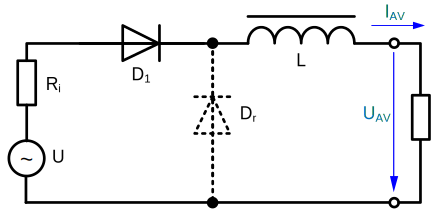
\includegraphics[width=0.6\linewidth]{patocka_jednocestny_1f_usm_LRzatez.pdf}
        \caption{Jednocestný jednofázový usměrňovač RL zátěží.}
        \label{enz:fig_usm_1f_RLz}
      \end{figure}

      \begin{itemize}\addtolength{\itemsep}{-0.5\baselineskip}
        \item Bude-li indukčnost veliká (v limitě nekonečná), pak podle Lenzova pravidla udrží  
              proud v obvodu (je celý v sérii) na stálé hodnotě i co do směru, dioda se nemůže 
              vůbec uzavřít a obvod nemůže usměrňovat - nebude mít střídavou složku.
        \item Naopak při malé hodnotě (proti jakési kritické) dioda zavře, obvod se přeruší a  
              energie magnetického pole cívky (je vázána existencí proudu) se nemůže uplatnit v 
              překlenutí mezer dodávky energie na výstup. Při dalším otevření diody můžou navíc 
              nastat přechodné děje.
      \end{itemize}

      Existuje však velice jednoduchá a plně funkční úprava a tou je doplnění jednocestného usměrňovače tzv. \textbf{rekuperační (nulovou) diodou} -
      $D_R$ (kreslena čárkovaně viz obr. \ref{enz:fig_usm_1f_RLz}). Při uzavření hlavní diody $D_1$ se tlumivka snaží držet proud obvodem ve stejné
      velikosti a ve stejném směru a tento proud otevře rekuperační diodu $D_R$.

      Mezi filtrací se sběrným kondenzátorem (RC zátěží) a s nárazovou tlumivkou (RL zátěží) je 
      ještě zajímavý rozdíl: filtrace paralelním kondenzátorem pracuje s hyperbolicky se měnící 
      impedancí $X_C=\frac{1}{\omega C}$ a potlačení vysokých čísel harmonických je čím dál tím 
      menší.  Obvod se sériovou tlumivkou pracuje s impedancí $X_L=\omega L$ a potlačující efekt 
      lineárně roste. \emph{Zvlnění na RC zátěži má proto obvykle dosti značný obsah vysokých 
      harmonických a je pilovitého průběhu. Zvlnění na RL zátěži je za stejných podmínek $K$ 
      harmonicky čistší a má charakter sinusovky.}


      % --------example: Usměrňovač --------------------------
      % \label{AES:exam001}
      % !TeX spellcheck = cs_CZ
\begin{example}\label{AES:exam001}
  Proveďte simulaci vyznačených obvodových veličin obvodu na obrá\-zku \ref{AES:fig_exam001_1} se 
  zadanými hodnotami prvků v programu  PSpice\footnote{Simulace je provedena v programu 
  \texttt{OrCAD PSpice} ver. 16.3}.

   {\centering
    \captionsetup{type=figure} 
    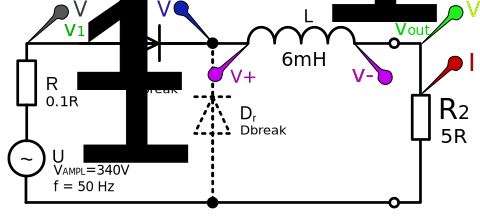
\includegraphics[width=0.8\linewidth]{patocka_jednocestny_1f_usm_PSpice.pdf}
    \captionof{figure}{Neřízený Jednofázový usměrňovač s nulovou diodu. Simulované veličiny jsou 
               vyznačeny barevnými markery.}
    \label{AES:fig_exam001_1}
    \par}

   {\centering
    \captionsetup{type=figure} 
    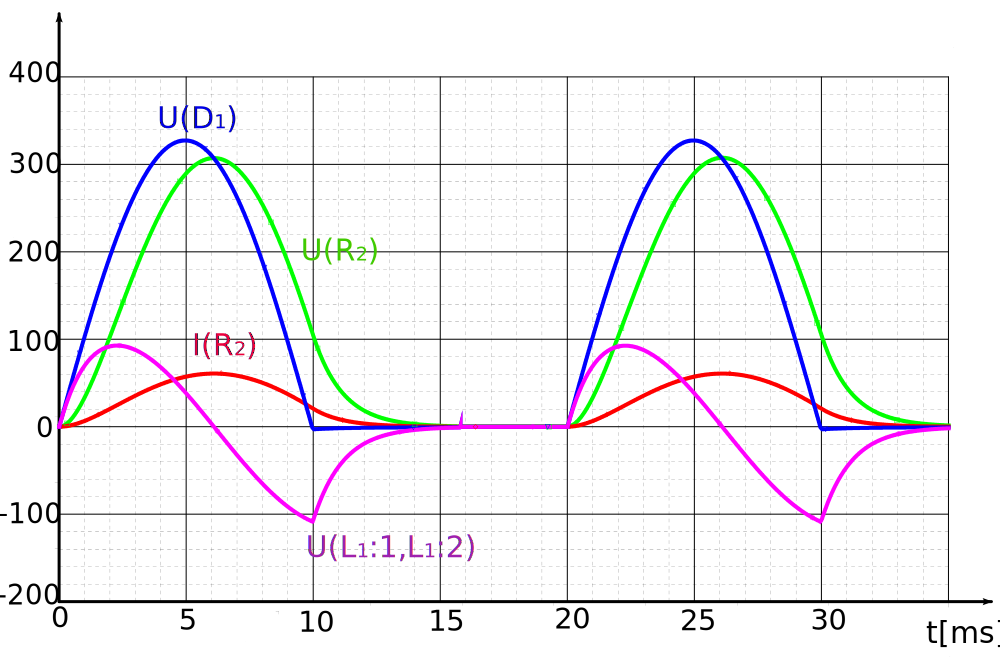
\includegraphics[width=0.9\linewidth]{PSPice_SIM002_usm1f_RL_6mH_5R.pdf}
    \captionof{figure}{Průběhy vyznačených veličin jednofázového neřízeného usměrňovače s RL zátěží 
              (6mH, 5$\Omega$) a nulovou diodou [ENZ/SIM002]}
    \label{AES:fig_exam001_2}
    \par}
\end{example}  
      %-------------------------------------------------------

  \section{Stabilizátory stejnosměrného napětí}
    Stabilizátory napětí na svém výstupu konstantní napětí v pokud možno co nejširším rozsahu 
    odebíraného výstupního proudu a dodávaného vstupního napětí \cite[s.~95]{Zahlava2001}
    \begin{itemize}
      \item nelineární (parametrické) stabilizátory napětí,
      \item lineární spojité stabilizátory napětí
    \end{itemize}

    \subsection{Nelineární (parametrické) stabilizátory}
      Využívají vlastností VA charakteristik některých jako je otevřený PN přechod, Zenerovy diody, termistory a jiné. Pro tyto účely potřebujeme tzv. prvky triodového typu u kterých platí, že \emph{dynamický vnitřní odpor je podstatně nižší jak statický}. Tedy $R_{dyn} < R_{stat}$. Pro naše účely jsou nejčastěji používané \emph{Zenerovy diody} a dvojpólové integrované \emph{napěťové referenční obvody}. Zenerovy diody jsou vyráběny jako malovýkonové ( anodová ztráta do 1W) a výkonové (obvykle 10W a více). Pro referenční účely jsou často doplněny dalšími pomocnými kompenzačními prvky. Vlastní princip nelineární\-ho spojitého stabilizátoru ( podivný název „parametrický“ nebudeme použí\-vat) je velice prostý: obvod dle obr. \ref{enz:fig_sch_ZD_stab} tvoří dělič s horním odporem lineárním a dolním (je paralelně k zátěži) tvořeným popsaným nelineárním odporem triodového typu. Za těchto okolností má tento obvod pochopitelně přenos dynamický podstatně menší jak statický a tedy je to stabilizátor napětí.

      \begin{figure}[ht!]
         \centering
         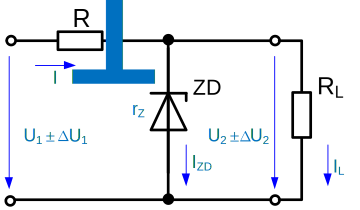
\includegraphics[width=0.6\linewidth]{patocka_stabilizator_ZD_sch.pdf}
         \caption{Nelineární spojitý stabilizátor napětí}
         \label{enz:fig_sch_ZD_stab}
       \end{figure}

      \begin{figure}[ht!]
         \centering
         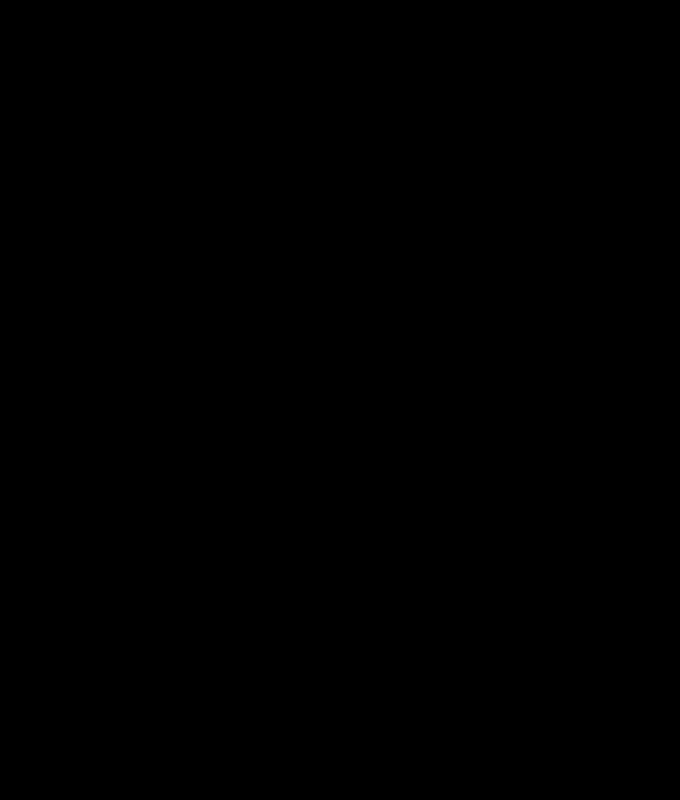
\includegraphics[width=0.8\linewidth]{patocka_stabilizator_ZD_VA.pdf}
         \caption{Grafické řešení nelineárního stabilizátoru}
         \label{enz:fig_graf_res_ZD_stab}
       \end{figure}

       Řešení je výhodné v grafické podobě - obr. \ref{enz:fig_graf_res_ZD_stab}. Ve třetím 
       kvadrantu je nakreslena VA charakteristika\footnote{Je typická určitým Zenerovým napětím 
       $U_z$, sklonem pracovní části VA charakteristiky (dynamickým vnitřním odporem  $r_z$) a 
       dovolenou anodovou ztrátou $P_{dov}$. Tato ztráta závisí na způsobu chlazení.} Bod 
       \texttt{B} odpovídá zvolenému vstupnímu napětí $U_1$ a výstupnímu proudu $I_2$ a tedy i 
       velikosti odporu $R_L$. Úloha může být nyní dána např. kolísáním vstupního napětí od 
       $U_{1_{max}}$ do $U_{1_{min}}$ (body \texttt{A} a \texttt{C}), nebo kolísáním zátěže nebo 
       proudu $I_2$ ( body \texttt{E'}a \texttt{D'}). Při současném působení změn vznikne obrazec 
       (přibližně obdélník) \texttt{X}, \texttt{E}, \texttt{D}, \texttt{H}, což je geometrické 
       místo možných stavů obvodů. Na vlastní VA charakteristice prvku pro volený "předřadný" odpor 
       \emph{R} vzniknou body \texttt{G}, \texttt{P} a \texttt{F} a to je grafické řešení. Vidíme, 
       kdy hrozí "zhasnutí" nebo přetíženi Zenerovy diody. Projekcí bodu \texttt{G}, \texttt{P} a 
       \texttt{F} na vodorovnou osu zjistíme okamžité hodnoty výstupního napětí stabilizátoru $U_2$ 
       a jeho kolísání $\Delta U_2$. Lze snadno odečíst zvládnutelné kolísání vstupního napětí či 
       velikosti zátěže atd. Z obrázku je také vidět, že zlepšení stabilizačního účinku obvodu lze 
       dosáhnout zvětšením vstupního napětí (větší odpor \emph{R}) nebo výběrem diody s menším 
       dynamickým odporem $r_z$ . Velice vtipná možnost zlepšení přenosových vlastností 
       stabilizátoru je při náhradě lineárního odporu \emph{R} nelineárním prvkem s pentodovým 
       charakterem VA charakteristiky. Může to být třeba bipolární nebo lépe unipolární tranzistor. 
       Pak vlastně Zenerovu diodu napájíme zdrojem konstantního proudu a to je hojně využívané v 
       integrovaných stabilizátorech.

       Z obr. \ref{enz:fig_sch_ZD_stab} lze snadno odvodit činitel napěťové stabilizace
       \begin{equation}\label{enz:eq_Su_ZD}
         S_u = \frac{\Delta u_{vst}}{\Delta u_{v\acute{y}st}} = \frac{R+r_z\parallel R_L}{r_z\parallel R_L} \cong \frac{R+r_z}{r_z}, \mathrm{kde} r_z\ll R_L
       \end{equation}

      % --------example: Stabilizátor ------------------------
      % \label{AES:exam002}
      % !TeX spellcheck = cs_CZ
\begin{example}\label{AES:exam002} Určete vliv nenulového dynamického odporu Zenerovy diody na 
  zvlnění výstupního napětí je-li zadáno: \(U_S = \SI{14}{\volt}, u_{ripple} = \SI{100}{\mV},
  U_Z = \SI{8}{\volt}, r_Z = \SI{10}{\ohm}, R_S = \SI{50}{\ohm}, R_L = \SI{150}{\ohm}\).
  \vspace{1em}
  
  {\centering
   \begin{tabular}{cc}
     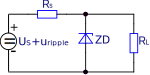
\includegraphics[width=0.4\linewidth]{stabilizator_ZD_ripple_effect.pdf}  &
     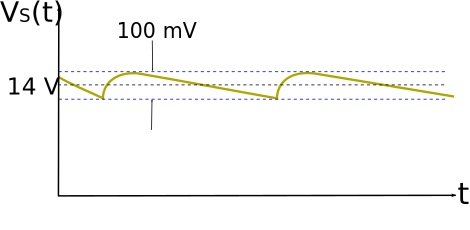
\includegraphics[width=0.5\linewidth]{stabilizator_ZD_ripple_graph.pdf}
   \end{tabular}
   \captionsetup{type=figure} 
   \captionof{figure}{K příkladu nenulového dynamického odporu Zenerovy diody na přenos zvlnění ze 
              vstupního napětí na výstupní napětí}
   \label{enz:fig_ZD_ripple}
 \par}
  \vspace{1em}
  \textbf{Řešení}:\newline Abychom stanovili velikost výstupního napětí, amplitudu zvlnění napětí 
  na zátěži a mohli také určit vliv velikosti dynamického odporu $r_z$, vyjděme z náhradního 
  lineárního obvodu na obrázku \ref{enz:fig_ZD_NLO}.
  \begin{enumerate}
    \item Stejnosměrný ekvivalentní obvod:
      \begin{align}\label{enz:eq_ZD_DC_UL}
         U_L &= U_S\frac{R_L\parallel r_z}{R_S + R_L\parallel r_z}   \nonumber \\
              + U_z\frac{R_S\parallel R_L}{r_z + R_S\parallel R_L}
             &= 2.21 + 6.32 = \SI{8.53}{\volt}
      \end{align}
    \item Střídavý ekvivalentní obvod:
      \begin{equation}\label{enz:eq_ZD_AC_UL}
        u_L = v_{ripple}\frac{r_z\parallel R_L}{R_S + r_z\parallel R_L} = \SI{16}{\mV}
      \end{equation}
      Tedy jedna šestina zvlnění vstupního napětí se přenese na výstupní svorky stabilizátoru.
  \end{enumerate}

  {\centering
   \begin{tabular}{cc}
     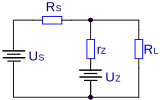
\includegraphics[width=0.4\linewidth]{stabilizator_ZD_DC_equival.pdf}
     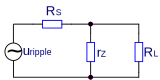
\includegraphics[width=0.4\linewidth]{stabilizator_ZD_AC_equival.pdf}
   \end{tabular}
   \captionsetup{type=figure} 
   \captionof{figure}{Stabilizátor se ZD lze pro výpočet jeho ss chování v okolí pracovního bodu  
            linearizovat pomocí NLO}
   \label{enz:fig_ZD_NLO}
  \par}
  Schopnost stabilizace je horší, čím větší má Zenerova dioda dynamický odpor $r_z$. Proto 
  musí být $r_z$ výrazně nižší, než hodnoty rezistorů $R_S$ a $R_L$ (viz rov. 
  \ref{enz:eq_ZD_AC_UL}).
\end{example}  
      %-------------------------------------------------------

    \subsection{Lineární spojité stabilizátory}
    
  \section{Násobiče napětí}
  \section{Ochranné a signalizační obvody zdrojů}
    \subsection{Pojistky}
       \subsubsection{Signalizace přerušené pojistky}
         Rozsvícením svítivé diody $D_1$, je uživatel upozorněn na přerušenou tavnou pojistku 
         $PO_1$ v zařízení napájeném malým napětím. Je-li pojistka v pořádku, je při zapnutém 
         vypínači $S_1$ na svítivé diodě napětí tvořené úbytky na pojistce a otevřené diodě $D_2$, 
         jenž nestačí pro její rozsvícení. Jakmile se však pojistka přeruší, dioda $D_1$ se 
         rozsvítí. Průchodu proudu spotřebičem přes $D_2$ při sepnutém vypínači $S_1$ brání její 
         polarizace.

         \begin{figure}[ht!]
           \centering
           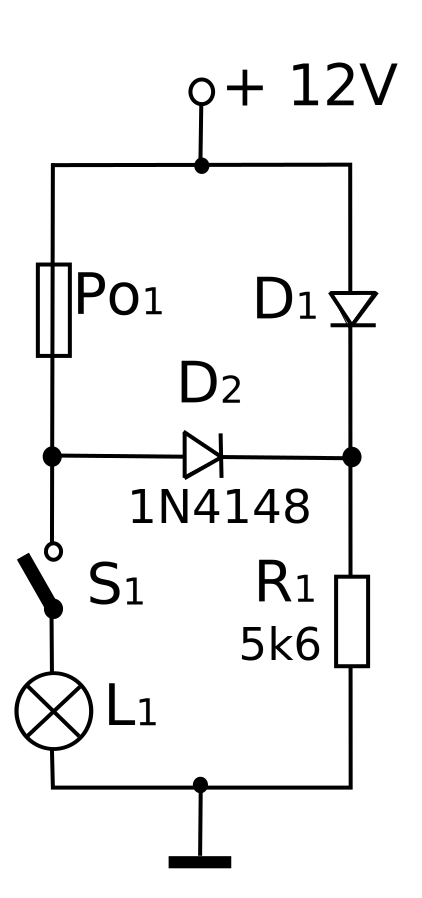
\includegraphics[width=0.4\linewidth]{sig_cir_fuse_failure.pdf}
           \caption{Obvod signalizující přerušení pojistky v nízkonapěťovém obvodu.}
           \label{enz:fig_fuse_failure}
         \end{figure}

} % tikzset
%---------------------------------------------------------------------------------------------------
\printbibliography[title={Seznam literatury}, heading=subbibliography]
\addcontentsline{toc}{section}{Seznam literatury}
